
%%%%%%%%%%%%%%%%%%%%%%% paper_sem_web.tex %%%%%%%%%%%%%%%%%%%%%%%%%
%
% This is the LaTeX source for the instructions to authors using
% the LaTeX document class 'llncs.cls' for contributions to
% the Lecture Notes in Computer Sciences series.
% http://www.springer.com/lncs       Springer Heidelberg 2006/05/04
%
% It may be used as a template for your own input - copy it
% to a new file with a new name and use it as the basis
% for your article.
%
% NB: the document class 'llncs' has its own and detailed documentation, see
% ftp://ftp.springer.de/data/pubftp/pub/tex/latex/llncs/latex2e/llncsdoc.pdf
%
%%%%%%%%%%%%%%%%%%%%%%%%%%%%%%%%%%%%%%%%%%%%%%%%%%%%%%%%%%%%%%%%%%%


\documentclass[runningheads,a4paper]{llncs}
\usepackage[utf8x]{inputenc}
\usepackage{amssymb}
\setcounter{tocdepth}{3}
\usepackage{graphicx}
\usepackage{footnote}
\usepackage{url}
\usepackage{subfigure} 
\urldef{\mailsa}\path|{manuel.b.dudda, robert.c.brylka, frank.b.reichwein,}@student.hs-rm.de|    
\newcommand{\keywords}[1]{\par\addvspace\baselineskip
\noindent\keywordname\enspace\ignorespaces#1}

\begin{document}

\mainmatter  % start of an individual contribution

% first the title is needed
\title{Semantic Web Technologien:\\FIFA's Fu\ss ball-Weltmeisterschaft 2014 in Brasilien bekommt eine semantische Unterst\"utzung.}

% a short form should be given in case it is too long for the running head
\titlerunning{Semantic Web: Brasil WM 2014}

% the name(s) of the author(s) follow(s) next
%
% NB: Chinese authors should write their first names(s) in front of
% their surnames. This ensures that the names appear correctly in
% the running heads and the author index.
%
\author{Manuel Dudda \and Robert Brylka\and Frank Reichwein}
%
\authorrunning{Brasil WM 2014 mit Semantic Web}
% (feature abused for this document to repeat the title also on left hand pages)

% the affiliations are given next; don't give your e-mail address
% unless you accept that it will be published
\institute{Hochschule RheinMain Informatik Master of Science \\
Fachbereich Design Informatik Medien \\
Campus Unter den Eichen 5
65195 Wiesbaden , Deutschland\\
\mailsa\\
\url{http://www.semanticwc.herokuapp.com}}

%
% NB: a more complex sample for affiliations and the mapping to the
% corresponding authors can be found in the file "llncs.dem"
% (search for the string "\mainmatter" where a contribution starts).
% "llncs.dem" accompanies the document class "llncs.cls".
%

\toctitle{Lecture Notes in Computer Science}
\tocauthor{Authors' Instructions}
\maketitle


\begin{abstract}
Große Sportereignisse haben schon immer große Menschenmassen begeistert. So auch die Events die die Disziplin Fußball betreffen. Dieses Paper beschreibt ein Projekt, das sich als Ziel die Präsentation der Ereignisse der diesjährigen FIFA Fußball-Weltmeisterschaft gesetzt hat. Der Fokus dieser Anwendung liegt auf der Aktualität der präsentierten Daten sowie einer auf mobile Endgeräte angepassten Repräsentation. Für die Vielfalt der Daten sowie deren Richtigkeit sorgt eine Informationssynthese aus mehreren Quellen. Um die Informationen weitestgehend für automatische Weiterverarbeitung vorzubereiten wurden alle Daten um semantische Bedeutung aus gängigen Sport-Ontologien ergänzt.
\end{abstract}

\section{Introduction}

In den vielen Informationsseiten, welche die diesjährige FIFA Fußball-Weltmeisterchaft in Brasilien präsentieren, sucht man oft vergeblich nach gut strukturierten und leichtgewichtigen Applikationen, die schnell mit mobilen Endgeräten zu erreichen sind. Zu dem werden viele Seiten nicht aktuell gehalten, was gerade bei so ereignisreicher Sportdisziplin wie Fußball unerlässlich ist. Bei unserem Projekt haben diese Aspekte die höchste Priorität erhalten. Um einem aktuellen Trend in der Webentwicklung zu folgen wurde unsere Applikation mit Konzepten des semantisches Web entwickelt. Dabei werden alle Informationen mit einer für die Maschine verständlicher Syntax ergänzt. Dazu wurden die Informationen der FIFA Webseite extrahiert und mit der Ontologie von BBC-Sport und der Ontologie Soccer-Voc des Hasso-Plattner-Instituts versehen. Für die Darstellung dieser Daten wurde eine Ruby on Rails Web-Applikation, welche zur Präsentation das jQuery Mobile Framework einsetzt, entwickelt. Des Weiteren werden weiterführende Informationen, durch die Einbeziehung von DBpedia Einträgen, eigeblendet.    


\section{Related Work}

Bei der Recherche in dem Bereich der Fußbaleregnisse mit semantischen Hintergrund hat sich unsere Aufmerksamkeit auf drei Quellen gerichtet, die Sport-Ontologie\footnote{\url{http://www.bbc.co.uk/ontologies/sport}} der BBC, die Soccer Voc Ontologie\footnote{\url{http://purl.org/hpi/soccer-voc/}} des Hasso-Plattner-Institut sowie der World Cup\footnote{\url{http://www.http://worldcup.sfg.io/}} JSON API.\\ Die Future Media and Technologie-Abteilung der BBC setzt auf semantische Technologien um die intern relevanten Inhalte automatisch verwalten zu können. Der erste große Einsatz der semantischen Technologien war die Gestaltung der Internetseite\footnote{\url{http://news.bbc.co.uk/sport2/hi/football/world_cup_2010/default.stm}} mit Informationen zu der FIFA Fußball-Weltmeisterschaft 2010. Die dabei eingesetzte Ontologie ist seither frei zugänglich. \\
Die Arbeitsgruppe "Semantic Technologies"\footnote{\url{http://hpi.de/meinel/knowledge_tech/semantics.html}} am Hasso-Plattner-Institut im Potsdam veröffentlichte 2012 ein Paper zu Linked Soccer Data\cite{url_lsd}. Im Rahmen dieses Papers wurde ein Datensatz mit Fußballinformationen vorgestellt, der mit der LOD Cloud\footnote{\url{http://linkeddata.org/}} verknüpft wurde. Die dabei verwendete Ontologie kann frei verwendet werden und stellt eine gute Ergänzung der Sport-Ontologie der BBC dar.\\
Bei der World Cup API handelt sich um ein von Eric Stiens\footnote{\url{http://softwareforgood.com/soccer-good/}} betreutes Projekt. Dessen Ziel ist es die aktuellen Fußballereignisse für jeden frei verfügbar zu machen. Neben der frei verfügbaren Informationen, die als JSON Dateien vorliegen, ist auch die API selbst für Weiterentwicklungen als Projekt\footnote{\url{https://github.com/estiens/world_cup_json/}} auf Github freigegeben. 


\section{Bestimmung der Informationsquellen}\label{infoQuell}

Die FIFA Fußball-Weltmeisterschaft ist allgemein ein belebtes Thema in der digitalen Welt. Um geeignete Quellen für die gesuchte Informationen zu finden wurde eine tiefgründige Recherche durchgeführt. Die unten aufgeführte Tabelle zeigt ein Ausschnitt aus der Zusammenstellung in der die Quellen aufgeführt wurden. Wie man an der Zusammenstellung erkennen kann verfügen nicht alle Quellen über die gleiche Informationsfülle. Dabei ist die Open Football Datenbank aufgrund der nicht aktuellen Informationen für weitere Verwendung uninteressant. Die Football Data sowie die World Cup Datenbank zeigen beide eine sehr gute Fülle an brauchbaren Informationen. Bei einer weiteren Recherche zu der Word Cup Datenbank wurde die offengelegte API gefunden, die einen direkten Zugriff auf die offizielle Seite der FIFA ermöglicht. Wie der letzten Spalte in der Zusammenstellung zu entnehmen ist, ist die offizielle Seite des internationalen Fußballverbandes die beste Informationsquelle. 
Daraus resultierend wurde ein Fork der Soccer for good API erstellt und dieser unseren Bedürfnissen angepasst. Durch die Anpassungen wurde die Schnittstelle um Informationen zu den Spielern, Trainern und Schiedsrichtern erweitert. Es wurden damit alle für die Anwendung relevaten Informationen  integriert. Dieser Fork bietet entsprechende REST\footnote{\textbf{Re}presentational \textbf{S}tate \textbf{T}ransfer} Endpunkte an. Die Rückgabe dieses Services ist eine JSON\footnote{\textbf{J}ava\textbf{S}cript \textbf{O}bject \textbf{N}otation}-Datei mit allen relevanten Informationen. \\


\begin{center}
%\begin{table}
\begin{savenotes}
\begin{tabular}{|l|c|c|c|c|c|}   \hline 
 & Football Data 	& Open Football 	& Footbal DB  &	World Cup  & FIFA  \\ \hline
References & \footnote{\url{https://github.com/footballdata/fifadata}} & \footnote{\url{https://github.com/openfootball/world-cup}
} &  \footnote{\url{http://footballdb.herokuapp.com/api/v1/}} &
 \footnote{\url{http://www.worldcup.sfg.io/}} & \footnote{\url{http://www.fifa.com/}} \\ \hline
 
Teams				& + & + & +	& + & +		\\ \hline
Gruppen				& - & + & -	& + & +		\\ \hline
Spiele				& + & + & -	& + & +		\\ \hline
Stadien				& + & + & -	& + & +		\\ \hline
Uhrzeiten			& + & + & -	& + & +		\\ \hline
Spieler				& + & + & - & - & +		\\ \hline
Spielergebnisse		& + & + & + & + & + 		\\ \hline
Torschützen/min		& +/+ & 	+/+ & - & + & +/+ 	\\ \hline
Schiedsrichter		& - & - & - & - & +		\\ \hline
Trainer				& - & - & - & - & +		\\ \hline
Spieltag 			& + & + & + & + & +		\\ \hline
Aktuell				& - & - & + & + & +  \\ \hline
Besucherzahl			& + & - & - & - & +		\\ \hline
			 
\end{tabular}

\end{savenotes}

%\label{tab:tab1} 

%\caption{Zusammenstellung der wichtigsten Informationsquellen}	
\end{center}


Eine wichtige Rolle bei der Wahl der API hat letztendlich auch der finanzielle Aspekt gespielt. Es gibt eine ganze Reihe an gut organisierten und stets aktuellen Datenbanken, die jedoch eine regelmäßige Gebühr mit sich tragen. Für dieses Projekt wurde jedoch die Vereinbarung getroffen, rein Quelloffene Lösungen zu verwenden. Dadurch wurden finanziell abhängige Projekte direkt bei der Recherche ausgeschlossen. 
  
\newpage
\section{Ontologien}
Um die Daten semantisch korrekt darzustellen wurden verschiedene Ontologien verwendet. Für die Darstellung der Weltmeistrschaft wurde die BBC-Sport-Ontologie verwendet. Mit dieser wurden die verschiedenen Gruppenphasen, Spieltypen, Spiele sowie die zugehörigen Stadien abgebildet. Für die Fußball spezifischen Daten wie Spielevents (Tore, Ein- und Auswechselungen sowie Karten) wurde die Soccer-voc-Ontologie des Hasso-Platner-Instituts verwendet. Diese erweitert die Friend of a Friend Ontolgie. Außerdem wurde die Event-Ontologie verwendet für die zeitliche Einordnung der Spielevents.

\begin{figure}
\centering
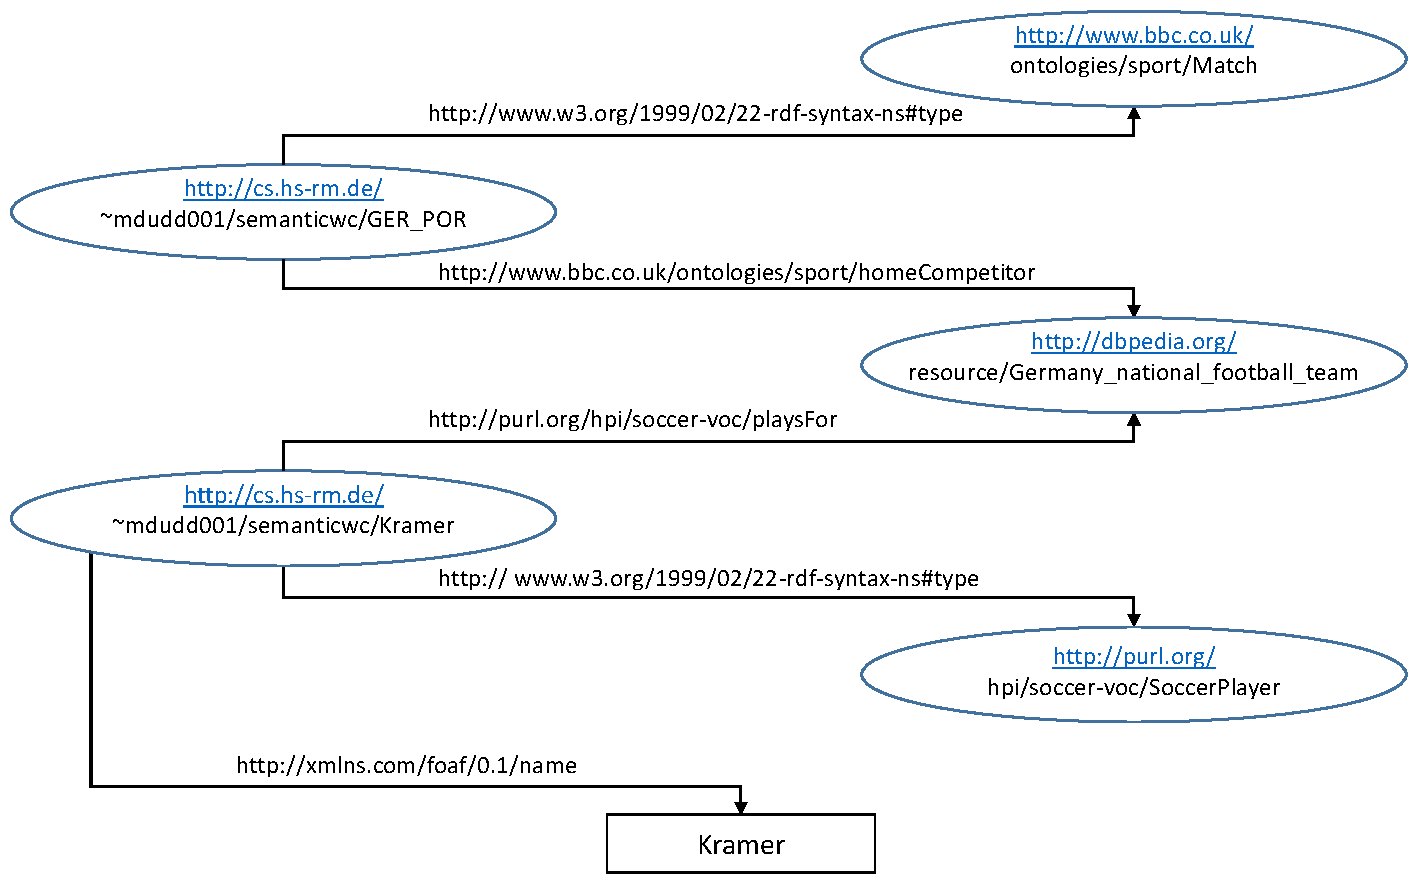
\includegraphics[height=7.2cm]{graph_manus}
\caption{Exemplarische Ausschnitt aus der RDF.}
\label{fig:onto}
\end{figure}

Die Abbildung \ref{fig:onto} zeigt einen Tripel-Graphen, der mit einen exemplarischen Ausschnitt aus der mit den Ontologien versehenen Daten, aufgebaut wurde. An diesem Beispiel ist die Verflechtung der Ontologien sehr gut sichtbar.
Aus den Tripeln ist ersichtlich, dass für jedes Spiel ein eigener Knoten mit den Länderkürzeln der Spielteilnehmer erstellt wurde \(GER\_POR\). Diese Subjekte sind vom Typ \textit{bbcsport:Match} und haben als \textit{bbcsport:homeCompetitior}-Prädikate die Objekte der jeweiligen Nationalmannschaft \(Germany\_national\_football\_team\). 
Des Weiteren gibt es einen Knoten für jeden Spieler, welche vom Typ \textit{soccer-voc:SoccerPlayer} sind. Diese sind mit dem Prädikat \textit{soccer-voc:playsFor} mit den Mannschaften verbunden. Das zuletzt genannte Prädikat und der zuletzt genannte Typ stammen von der Soccer-voc Ontologie. Da \textit{SoccerPlayer} eine Unterklasse von \textit{foaf:Agent} ist, kann ein SoccerPlayer mit einem Prädikat der FOAF-Ontolgie für einen Namen versehen werden.
\newpage
\section{Application \& Implemetierung}


Bei der Wahl des Framework für diese Anwendung fiel die Entscheidung zu Gunsten von Ruby on Rails \footnote{http://www.rubyonrails.org/} aus. Durch die verfügbaren Erweiterungen bietet es eine sehr gute Unterstützung bei Entwicklung von Semantik Web Applikationen. Sei es bei dem erzeugen von RDF Daten oder den SPARQL-Abfragen. Für die Gestaltung der Seiten sowie als Unterstützung für die Mobilen-Endgeräte wurde die jQuery Mobile\footnote{http://www.jquerymobile.com/} Bibliothek eingesetzt. Durch diese Bibliotheck werden auf Mobilen-Endgeräten z.B. Swipe-Gesten unterstützt. 

\begin{figure}
\centering
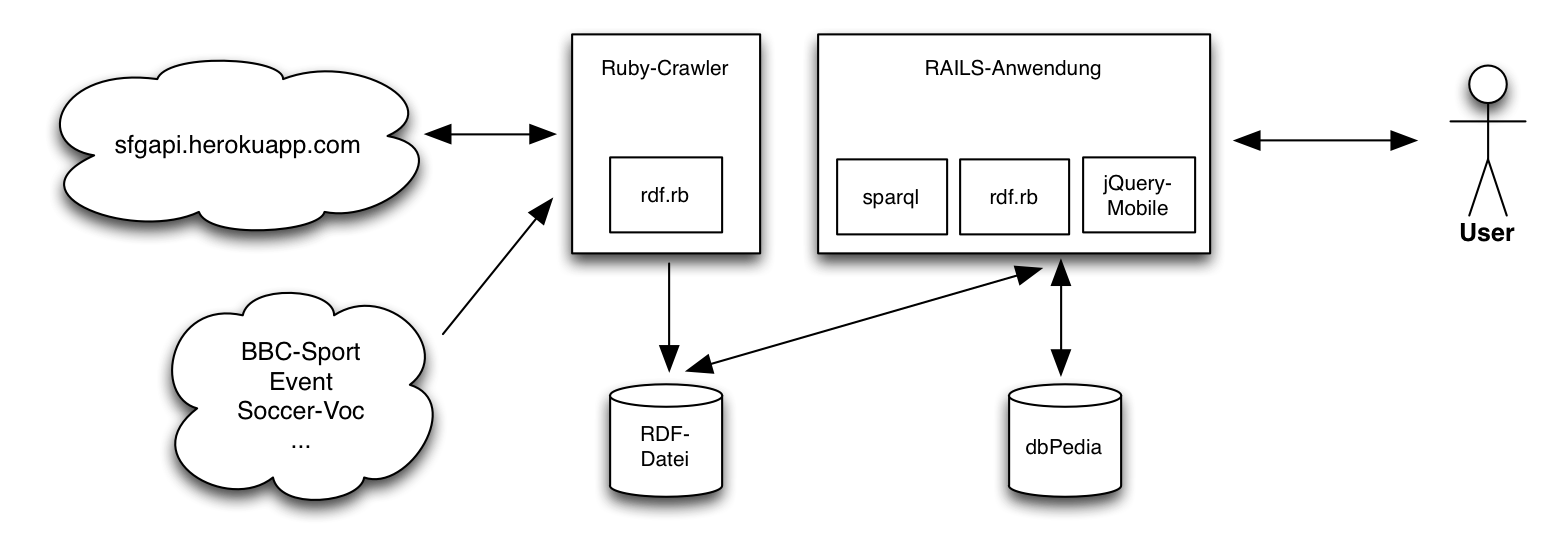
\includegraphics[height=3.2cm]{technik-stack}
\caption{Technik-Stack}
\label{fig:example}
\end{figure}

Die Abbildung \ref{fig:example} zeigt eine Übersicht über den Technik-Stack. Die Applikation wurde in drei Bereiche eingeteilt. Ein REST-Endpunkt, ein Crawler und die Ruby on Rails Applikation welche für die Präsentation der Daten zuständig ist.

Die Ruby on Rails Applikation welche die Informationen der FIFA-Seite crawlt und diese in einem REST-Endpunkt zuverfügung stellt, ist ein Fork des Soccer for good\footnote{\url{https://github.com/estiens/world_cup_json/}} Projektes. Der entwickelte REST-Endpunkt ist auch separat über \texttt{sfgapi.herokuapp.com} erreichbar. Der Service wurde erweitert, indem die Aufstellung der Mannschaften, Trainer sowie die Schiedsrichter für jedes Spiel angezeigt werden. 

Als zweiter Teil der Anwendung wurde ein Crawler implementiert. Der Crawler benutzt die Informationen der REST-API, versieht diese mit den passenden Ontologien und erstellt einen Graphen. Für die Erstellung des Graphen wird das Ruby Gem rdf.rb\footnote{\url{https://github.com/ruby-rdf/rdf}} benutzt. Da die Anwendung sich zunächst auf ein Sportliches Ereignis beschränkt, in diesem Fall die Fußballweltmeisterschaft, wurde für speicherung keine zusätzliche Datenbank verwendet. Stattdessen werden alle Datensätze als RDF-Tripel in einer Datei (\textit{worldcup.ttl})gespeichert. Für die Serialisierung der Datenbestände wurde hierbei Turtle Syntax verwendet. Diese Datei enthält über 10.000 Triple und ist ca. 900 KB groß, da durch kann der komplette Datenbestand, ohne Probleme, im RAM gehalten werden.
\newpage

Für die Präsentation der Ergebnisse ist eine Ruby on Rails App entwickelt worden, die zur Darstellng jQuery-Mobile verwendet. Für die Darstellung wurden verschiedene SPARQL-Abfragen erstellt, um die entsprechenden Informationen aus der Datei zu extrahieren. Da die Informationen in der Datei mit DBpedia verknüpft sind, mussten außerdem SPARQL-Abfragen für den SPARQL-Endpunkt von DBpedia entwickelt werden. Die Anwendung stellt alle Spiele mit Ergebnissen, Toren und Torschützen da. Außerdem gibt es für jede Mannschaft eine Ansicht welche den Kader darstellt. Die Informationen zu den jeweiligen Spieler kommen von DBpedia. Des weiteren gibt es eine Ansicht der Stadien, welche die Position des Stadions mittels Google-Maps darstellt. Die Geo-Position der Stadien wirde ebenfalls bei DBpedia abgefragt.

\begin{figure}
\centering
\subfigure[Spiele-Ansicht]{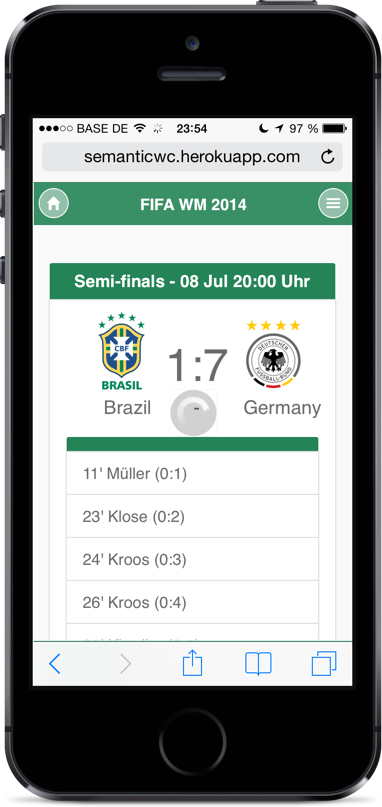
\includegraphics[height=6.19cm]{screenshots/matches_view}\label{fig:matches_view}} 
\subfigure[Spiele-Filter]{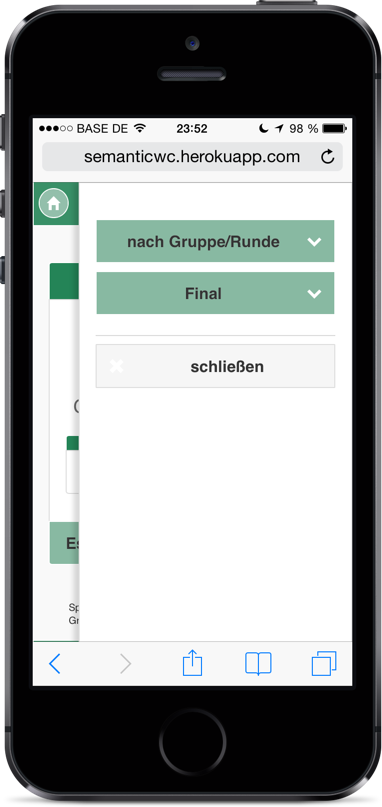
\includegraphics[height=6.19cm]{screenshots/matches_filter_view}\label{fig:matches_filter_view}}
\subfigure[App im Einsatz]{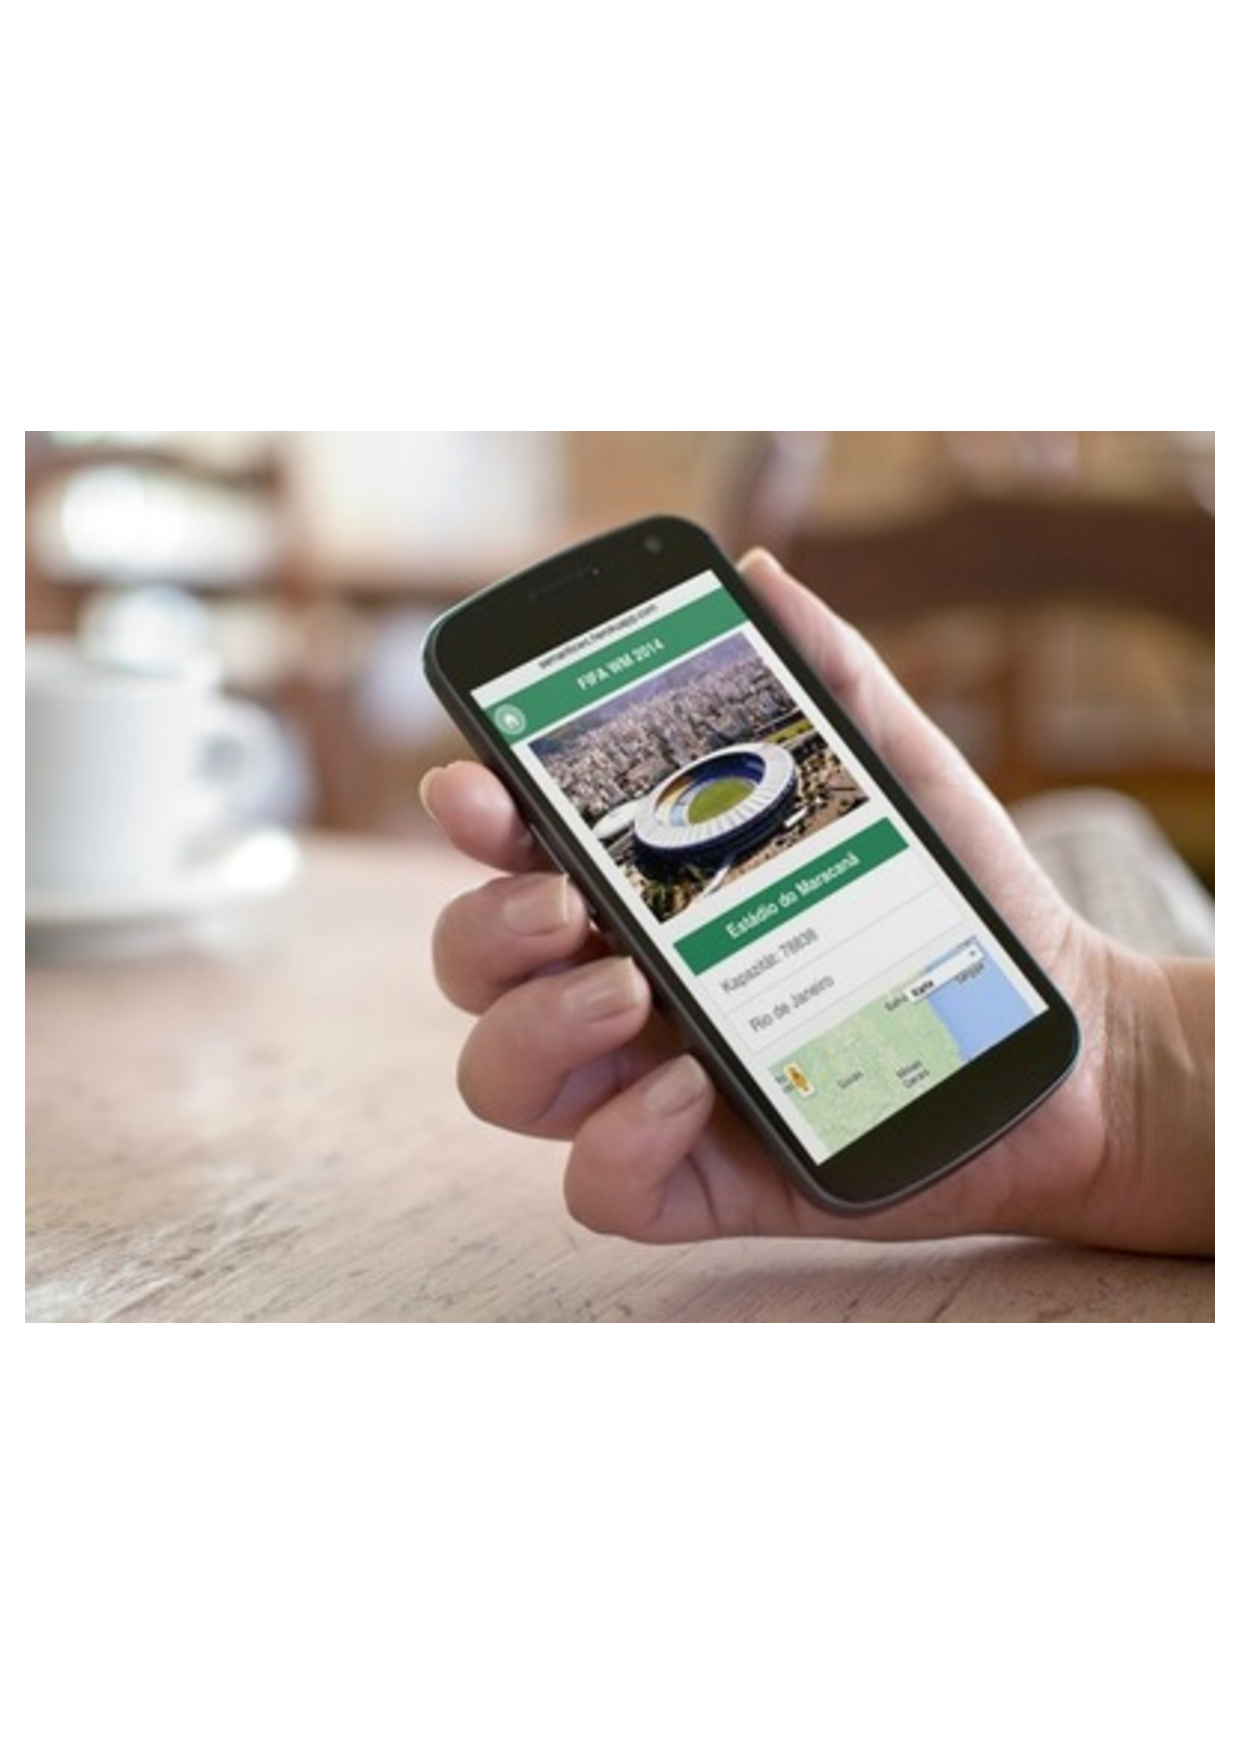
\includegraphics[height=6.19cm]{screenshots/android}\label{fig:android}}
\caption{Multi-Views}
\label{fig:screenshots}
\end{figure}

In der Abbildung \ref{fig:screenshots} sind mehrere Screenshots aus unterschiedlichen Ansichten der Anwendung zu sehen. In Abb. x ist die Startseite zu sehen, auf der immer der aktuelle Spieltag anzeigt wird. Abb. xx ist ein Ausschnitt aus der Ansicht, die Informationen zu Stadien präsentiert. Abb. xxx zeigt wiederum eine Ansicht die die Informationen zu einem Trainer einer Mannschaft präsentiert. Da die Anwendung vorwiegend auf mobile Endgeräte ausgelegt ist, wurde bei der Gestaltung der einzelnen Ansichten ein großer Wert auf die Übersichtlichkeit gelegt. Für eine schnelle Navigation wurden zudem zwei Buttons eingepflegt. Der 'Home' Button, der in jeder Ansicht in der oberen linke Ecke zu sehen ist, führt immer zu der Seite mit den aktuellen Spieltag. Mit dem 'Bar' Button, in oberen rechten Ecke der Spiele Ansicht, kann eine Seitenansicht mit mehreren Filteroptionen eingeblendet werden. Dabei kann der Inhalt nach dem Team, der Gruppe/Runde, dem austragenden Stadion oder dem Datum sortiert werden.

\begin{figure}
\centering
\subfigure[Stadion-Ansicht]{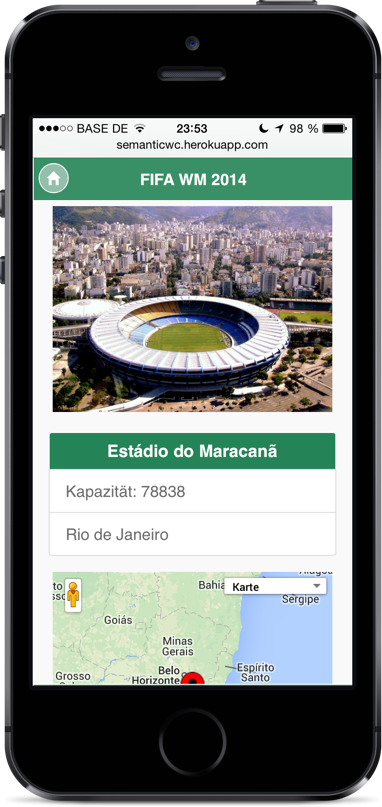
\includegraphics[height=6.19cm]{screenshots/stadium_view}\label{fig:stadium_view}} 
\subfigure[Team-Ansicht]{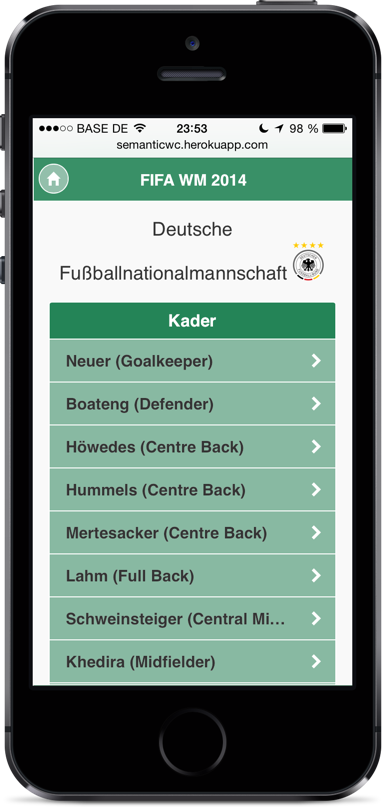
\includegraphics[height=6.19cm]{screenshots/team_view}\label{fig:team_view}}
\subfigure[Spieler-Ansicht]{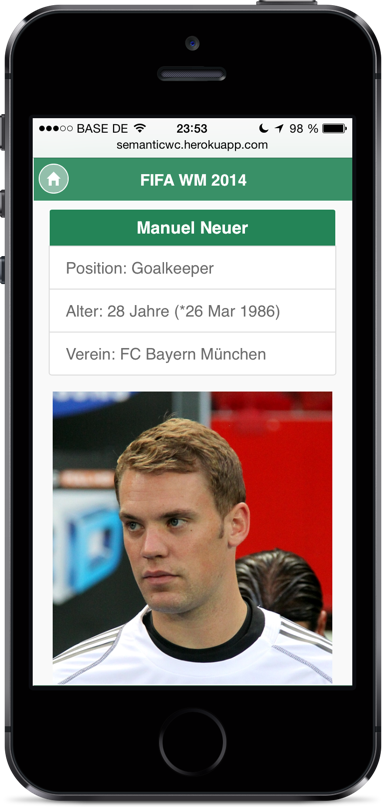
\includegraphics[height=6.19cm]{screenshots/player_view}\label{fig:player_view}}
\subfigure[Trainer-Ansicht]{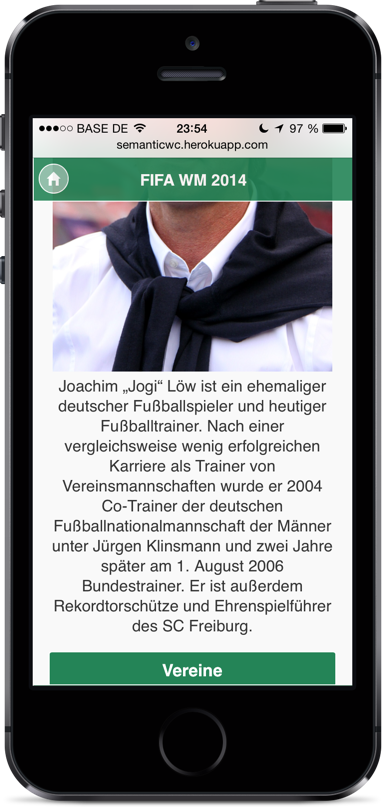
\includegraphics[height=6.19cm]{screenshots/trainer_view}\label{fig:trainer_view}}
\caption{Single-Views}
\label{fig:screenshots2}
\end{figure}
       

%In den folgenden Abbildungen sind mehrere Screenshots aus unterschiedlichen Ansichten der Anwendung zu sehen. In Abbildung \ref{fig:matches_view} ist die Startseite zu sehen, auf der immer der aktuelle Spieltag anzeigt wird. Abb. \ref{fig:stadium_view} ist ein Ausschnitt aus der Ansicht, die Informationen zu Stadien präsentiert. Abb. \ref{fig:trainer_view} zeigt wiederum eine Ansicht die die Informationen zu einem Trainer einer Mannschaft präsentiert. Da die Anwendung vorwiegend auf mobile Endgeräte ausgelegt ist, wurde bei der Gestaltung der einzelnen Ansichten ein großer Wert auf die Übersichtlichkeit gelegt. Für eine schnelle Navigation wurden zudem zwei Buttons eingepflegt. Der 'Home' Button, der in jeder Ansicht in der oberen linke Ecke zu sehen ist, führt immer zu der Seite mit den aktuellen Spieltag. Mit dem 'Bar' Button, in oberen rechten Ecke der Spiele Ansicht, kann eine Seitenansicht mit mehreren Filteroptionen eingeblendet werden (Abb. \ref{fig:matches_filter_view}). Dabei kann der Inhalt nach dem Team, der Gruppe/Runde, dem austragenden Stadion oder dem Datum sortiert werden.

Aus der Hauptansicht, in der immer der aktuelle Spieltag angezeigt wird, kann mit einer Wischgeste nach links oder rechts zu den bereits stattgefundenen, respektive in der Zukunft liegenden Spielen gewechselt werden. Die gleiche Funktionalität liegt auch bei der Ansicht, die durch Anwenden der Filteroperation \textit{nach Team}, \textit{nach Stadion}, \textit{nach Gruppe/Runde} sowie \textit{nach Tag} gewählt wird.
In den Single-Views (Abb. \ref{fig:screenshots2}) kann mit einer Wischgeste von links nach rechts zurück navigiert werden.

\newpage

\section{Zusammenfassung und Ausblick}

Im Rahmen dieses Projekts wurde eine Anwendung entwickelt, die alle wichtigen Informationen, zu der 2014 in Brasilien stattfindenden FIFA Fußball-Weltmeisterschaft, bereithält. Als Informationsquelle dient hierbei die offizielle FIFA Webseite, die mit Daten aus der DBpedia ergänzt wurde. Die semantische Aufbereitung wurde mit Hilfe der BBC Sport sowie der Socker Voc Ontologie gestaltet.  

Unsere Anwendung bietet eine solide Grundlage für Weiterentwicklungen die nicht nur den Bereich Fußball betreffen. Bezogen auf die Fußballereignisse kann eine leichte Portierung auf die nächste Weltmeisterschaft oder Europameisterschaft stattfinden. Denkbar ist aber auch eine Abwandlung zur Informationspräsentation der Spiele der nationalen Meisterschaften, beispielsweise der Fußball-Bundesliga.

Die Struktur- und Spieldaten der Weltmeisterschaft umfasst über 10000 RDF-Tripel. Diese sind weitestgehenst mit DBpedia-URIs verknüpft. Für die Datenabfragen wurden über 200 Zeilen Sparqlcode implementiert. Leider ist eine Zuverlässigkeit von DBpedia nicht garantiert. Während der Implementierungsphase mussten wir Änderungen am Sparql-Enpoint feststellen, die zum Ausfall der Applikation führte. Des Weiteren hat man immer wieder mit unangekündigten Wartungsarbeiten sowie Performanceproblemen seitens DBpedia zu kämpfen. Unserer Einschätzung steht dieses Projekt noch in den Kinderschuhen - die Daten sind veraltet, Attribute werden inkonsistent mit Prädikaten versehen, Sprachattribute sind oftmals falsch. So enstanden große, unübersichtliche SPARQL-Abfragen, die auf viele optionale Prädikate der gleichen Semantik abzielen. Dieser Umstand ist insbesondere bei Namen zu beobachten, die bis zu 10 verschiedene Prädikate aus 5 Ontologien berücksichtigen. Die Qualität und Verfügbarkeit der Daten ist inkonsistent und führt nur durch heuristische Mittel zu akzeptablen Ergebnissen.



\begin{thebibliography}{4}

\bibitem{url_lsd}Linked Soccer Data,
Tanja Bergmann, Stefan Bunk, Johannes Eschrig, Christian Hentschel, Magnus Knuth, Harald Sack, and Ricarda Schüler\\
Hasso Plattner Institute for Software Systems Engineering, Potsdam, Germany\\
Letzter Zugriff: 22. Juni 2014\\
\url{http://ceur-ws.org/Vol-1026/paper6.pdf}

\bibitem{url_bbc}BBC ONTOLOGIES, A simple ontology for representing competitive sports events.\\
Letzter Zugriff: 26. Juni 2014\\
\url{http://www.bbc.co.uk/ontologies}

\bibitem{url_jquery}jQuery mobile,
Letzter Zugriff: 26. Mai 2014\\
\url{https://demos.jquerymobile.com/1.4.2/}

\bibitem{url_smm}Semantic Media Mining,\\
Letzter Zugriff: 22. Juli 2014\\
\url{https://smm2013.blogspot.de/2012/11/soccer-voc.html}

\bibitem{url_dbpedia}DBpedia,
Letzter Zugriff: 22. Juli 2014\\
\url{http://http://dbpedia.org}

\bibitem{url_ruby}Ruby. Der beste Freund eines Programmierers,
Letzter Zugriff: 22. Juli 2014\\
\url{https://www.ruby-lang.org/de/}

\end{thebibliography}


\end{document}
